\documentclass[11pt]{article}
\setlength{\textheight}{240mm}
%\setlength{\voffset}{0mm}
\addtolength{\topmargin}{-30mm}
\setlength{\textwidth}{155mm}
\setlength{\oddsidemargin}{5mm}
\usepackage{graphicx, subfig}
\graphicspath{ {./figs} }
\pagestyle{plain}
\begin{document}
\title{Preferential Attachment Coarse Projective Integration}
\author{Alexander Holiday\vspace{-2ex}}
\date{09/01/2013}
\maketitle
\section*{Introduction}
The edge reconnecting model, detailed in \cite{balasz:rsa12}, was implemented in C++. The system naturally converges to a limiting ``graphon'' (see \cite{lovasz:jcombth06}), and in order to increase the rate of convergence, coarse projective integration (CPI) was implemented. This brief outlines the model dynamics and reviews current simulation progress.

\section*{Edge Reconnecting Model}
The initial state of the edge reconnecting model is an Erd\H{o}s-R\'{e}nyi random graph with $n$ vertices and $m\sim O(n^{2})$ edges. The system evolves as a discrete-time Markov chain, in which the followinnng actions are performed during each step:

\begin{enumerate}
\item An edge $e_{old}$ is chosen uniformly at random from the set of all possible edges, $E(G)$.
\item A vertex end of $e_{old}$, $v_{1}$, is chosen uniformly from the two ends.
\item $e_{old}$ is removed from the graph, and a vertex $v_{2}$ is chosen from $V(G)$ with a probability determined based on linear preferential attachment:
  \[
  P(v_{2}=v_{i})=\frac{deg(v_{i})+\kappa}{2m+n\kappa}
  \]
where $\kappa$ is a model parameter and $deg(v_{i})$ denotes the degree of vertex $i$ in $V$.
\item An edge $e_{new}$ is added between $v_{1}$ is connected to $v_{2}$.
\end{enumerate}

Two distinct timescales arise from these dynamics, $T\asymp n^{2}$ and $T\asymp n^{3}$ where $T$ is the number of steps. On the faster, $O(n^{2})$ scale, the degrees of the vertices may be considered constant, while the number of parallel edges between vertices changes. On the slower $O(n^{3})$ scale, the degree distribution evolves to a steady state value. While this separation of timescales has been proven on in \cite{balasz:rsa12}, identifying them through numerical simulations is complicated by a couple of factors. First, the exact timescales themselves are difficult to discern. Both scales are really $O(\rho_{1} n^{2})$ and $O(\rho_{2} n^{3})$, where the $\rho_{i}$ constants are evaluated at the limit of infinite-sized graphs ($n\rightarrow \infty$). This hints at the second, larger, problem: many of the results on the existence of these timescales in the first place are only valid in this large-$n$ limit. Simulation time then becomes problematic. \ref{fig:degSurf100} and \ref{fig:degSurf500} illustrate attempts to visualize these separate scales of evolution.

\begin{figure}
  \centering
  \subfloat[$n=100$] {
    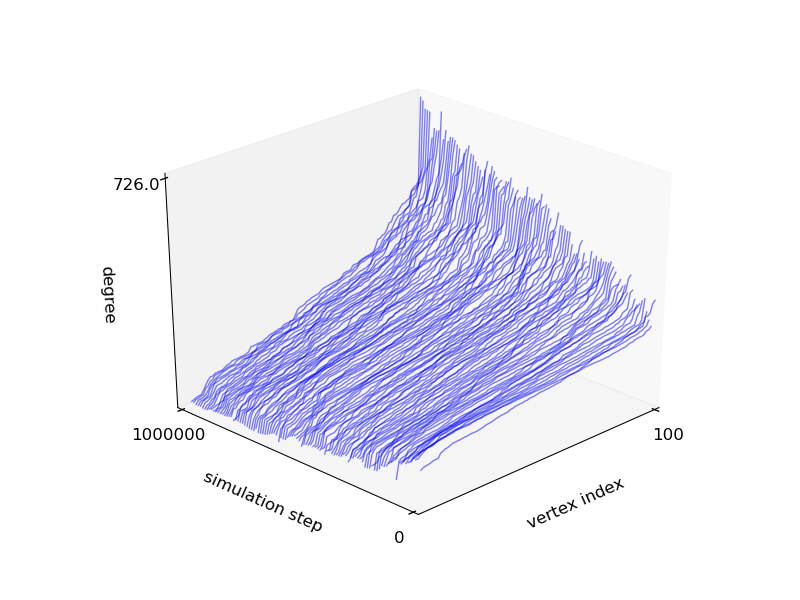
\includegraphics[width=72mm]{degSurf100}
    \label{fig:degSurf100}
  }
  \subfloat[$n=500$] {
    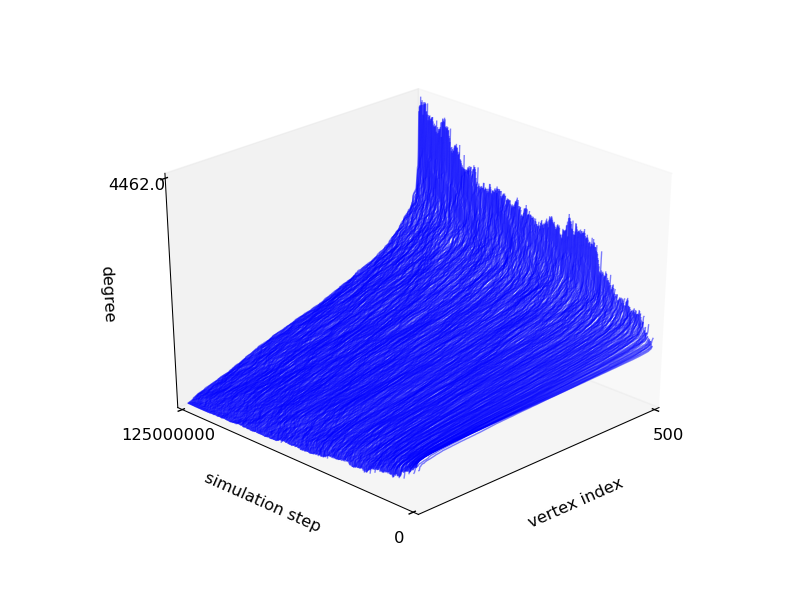
\includegraphics[width=72mm]{degSurf500}
    \label{fig:degSurf500}
  }
  \caption[Evolution of degree distribution for $n^{3}$ steps]
\end{figure}

\end{document}
